%% implemen.tex
%% $Id: implemen.tex 61 2012-05-03 13:58:03Z bless $
%%

\chapter{Implementierung}
\label{ch:Implementierung}
%% ==============================

Aufgrund der unterstützenden Funktionen, wie das Portieren auf verschiedene Systeme, habe ich mich für die Unity Engine in der Version 2019.3.14f entschieden, um Latrunculi digital umzusetzen. Die Erklärung zu Unity befindet sich im Abschnitt \ref{ch:Grundlagen:sec:Unity}. Weiterhin habe ich mich in C\# eingearbeitet und damit die verwendeteten Skripte geschrieben und genutzt. Da ich vorher noch nicht mit Unity und C\# gearbeitet habe, benötigte ich etwas Einarbeitungszeit um den ersten Prototypen zu erstellen.

%\begin{figure}[h]
%	\centering
%	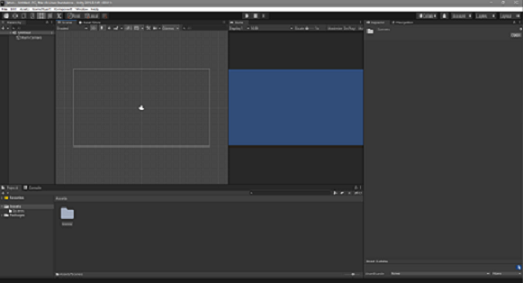
\includegraphics{img/Unity-Editor}
%	\caption{Unity-Editor}
%	\label{fig:Editor}
%\end{figure}

%% ==============================
\section{Unity}
%% ==============================
\label{ch:Implementierung:sec:Unity}

Die ersten Versuche einer lauffähigen Umsetzung habe ich mit einem vorgefertigten Spielbrett umgesetzt. Dabei habe ich das Brett durch 8x8 einzelne Zellen beziehungsweise Quadrate dargestellt. Auf diesen Quadraten habe ich die Spielsteine als schwarze und graue Kreise platziert und diesen via Skript Funktionen gegeben. Dieser erste Entwurf (Abbildung \ref{fig:Prototyp}) reagierte auf das OnClick()-Event, sodass beim Anklicken eines Kreises der mögliche Weg hervorgehoben wurde und beim Klick auf das gewünschte Feld, wurde der Kreis auf diesem neuen Feld platziert.
Da dieser Entwurf sehr statisch und die Größe fest verankert war, habe ich mir Informationen gesucht um das Spiel dynamisch zu erstellen und die Größe des Spielfelds variabel zu machen. Dazu habe ich sowohl für die Zellen, als auch die Spielsteine Prefabs erstellt und somit mittels Skript in der Start-Funktion die Prefabs abgerufen und je nach angegebener Größe das Spielfeld zur Laufzeit erstellt.
Außerdem wurde das OnClick()-Event durch Drag \& Drop ersetzt, sodass es auf einem Touchscreen intuitiver zu bedienen ist.
%% ==============================
\section{GameObjects}
%% ==============================
\label{ch:Implementierung:sec:GameObjects}
Um die einzelnen Spielelemente darzustellen, müssen im Unity-Editor erst Spielobjekte (englisch: GameObject) erstellt werden. Die folgenden Objekte wurden dem Spiel hinzugefügt:
\paragraph{Main Camera}
Die Kamera ist zuständig für das Sichtfeld, sodass hier festgelegt werden kann, was innerhalb der Szene sichtbar ist.
\paragraph{Board}
Das \textbf{Board} ist das Objekt, dass das Spielbrett darstellt. Via Prefabs werden dem Board zur Laufzeit die einzelnen Zellen hinzugefügt und so das Brett aufgebaut.
\paragraph{PieceManager}
Der \textbf{PieceManager} ist zuständig für die einzelnen Spielsteine, die ebenfalls via Skript und Prefab der Szene und dem PieceManager hinzugefügt werden.
\paragraph{GameManager}
Der \textbf{GameManager} beinhaltet die Spiellogik und lässt das Spiel starten, sowie auch beenden. Hier wird nach jedem Zug geprüft ob ein Spieler gewonnen hat oder das Spiel noch weiter läuft. Weiterhin wird hier die Berechnung der KI angestoßen.
\paragraph{EscapeMenuManager}
Der \textbf{EscapeMenuManager} ist zuständig für das Event-Handling des Menüs und der Buttons. Das heißt, hier wird entschieden, ob das Menü sichtbar und was in dem Menü zu sehen ist.

%% ==============================
\section{Skripte}
%% ==============================
\label{ch:Implementierung:sec:Skripte}
Damit die einzelnen Objekte auch Funktionen und Informationen bekommen, musste jedem Objekt ein Skript hinzugefügt werden.
Beispielsweise hat jeder Spielstein das Skript \textbf{SimplePiece} zugeordnet bekommen. Dieses ermöglicht dem Spielstein die Bewegungen auf dem Spielbrett durchzuführen. Es enthält Funktionen die auf das Ein- und Austreten des Drag\&Drop-Events reagieren. Des Weiteren werden hier Informationen über die Ursprungszelle, sowie die aktuelle Zelle gespeichert um das Zurücksetzen des Spiels für einen Neustart nach dem Beenden eines Spiels zu vereinfachen. \\
Das \textbf{PieceManager}-Skript ist für die Spielsteine insgesamt zuständig, das heißt hier werden die Prefabs und Skripte der Spielsteine instanziiert und der Szene hinzugefügt beziehungsweise auf dem Spielbrett platziert. Außerdem kann dieser Manager die Funktionen der Spielsteine ein und ausschalten, sodass nur mit den Steinen interagiert werden kann, die auch gerade am Zug sind, vorausgesetzt das Spiel befindet sich nicht im Simulations-Modus.\\
Der \textbf{EscapeMenuActivator} ist für das Ein- und Ausschalten des Menüs zuständig.\\
Der \textbf{GameManager} stößt jeden Spiel-relevanten Prozess an, speichert ob eine oder zwei KIs aktiviert sind und lenkt dementsprechend das Spielgeschehen. Das Spiel wird hier auch gestartet und beendet.\\
Das Spielbrett erhält das \textbf{Board}-Skript und initiiert den Aufbau des Spielbretts. Außerdem werden hier alle Zellen und deren Anordnung gespeichert, sodass das Board mögliche Züge validieren kann.\\
Für die Berechnungen der KI erbt das Skript \textbf{BoardDraught} die Funktionen und Variablen des Board-Skriptes, übernimmt aber nur die wichtigen Informationen.\\
Jede Zelle erhält ebenfalls ein eigenes Skript (\textbf{Cell}), dass die Position der Zelle beinhaltet und den Spielstein, der sich auf der Position befindet. Außerdem wird hier das Hervorheben der Zellen durchgeführt.\\
Die Klasse \textbf{Move} enthält Informationen für eine mögliche Bewegung, das heißt hier wird die aktuelle Position des gerade betrachteten Spielsteins gespeichert, sowie die Zelle auf welche sich der Stein bewegen kann. Weiterhin enthält diese verschiedene Flags, die zur Bewertung der Aktion dienen.\\
Im \textbf{AIManager} befindet sich der MiniMax-Algorithmus, der die Berechnungen und Bewertungen der möglichen Züge durchführt. Wie genau der Algorithmus funktioniert wird im nachfolgenden Abschnitt erklärt.

%% ==============================
\section{MiniMaxing}
%% ==============================
\label{ch:Implementierung:sec:MiniMaxing}
Für die Implementierung des MiniMax-Algorithmus habe ich die Klasse AIManager entworfen. Diese enthält die Funktion \textbf{Minimax()}, die sich an der beschriebenen Umsetzung von Jorge Palacios\cite{palacios2016unity} orientiert. Diese übernimmt das aktuelle Spielbrett als Board, die maximale Suchtiefe, die aktuelle Tiefe und den Spieler der am Zug ist. Die Berechnungen und Evaluation der möglichen Züge werden anschließend hier rekursiv durchgeführt und es wird die maximal erreichte Punktzahl zurückgegeben, sowie die Referenzierung des zugeordneten Zuges.\\
\begin{figure}[h]
\begin{lstlisting}[basicstyle=\scriptsize\ttfamily, numbers=left, stepnumber=1, numberstyle = \tiny]
public static float Minimax(BoardDraught board, int player, int maxDepth,
int currentDepth, ref Move bestMove)
{
	if (board.IsGameOver() || currentDepth == maxDepth)
		return 0;
	bestMove = null;
	float bestScore = Mathf.Infinity;
	if (board.GetCurrentPlayer() == player)
	bestScore = Mathf.NegativeInfinity;
	List<Move> allMoves = new List<Move>();
	int nextPlayer = 0;
	if (player == 2){
		allMoves = board.GetMoves(player);
		nextPlayer = 1;
	}
	else if (player == 1){
		allMoves = board.GetMoves(player);
		nextPlayer = 2;
	}
	Move currentMove;
	float score = 0;
	foreach (Move m in allMoves){
		board.MakeMove(m);
		float currentScore = 0;
		currentMove = m;
		if (m.attacked)	{
			if (nextPlayer == 2)
			nextPlayer = 1;
			else
			nextPlayer = 2;
		} 
		currentScore = Minimax(board, nextPlayer, maxDepth, 
				currentDepth + 1, ref currentMove);
		float newScore = board.Evaluate(player);
		if (board.GetCurrentPlayer() == player)	{
			currentScore += newScore;
			if (currentScore > bestScore)
			{
				bestScore = currentScore;
				bestMove = m;
				m.mScore = bestScore;
			}
		}
		else{
			currentScore -= newScore;
			if (currentScore < bestScore){
				bestScore = currentScore;
				bestMove = m;
				m.mScore = bestScore;
			}
		}
		board.StepBack();
		if (m.attacked){
			if (nextPlayer == 2)
				nextPlayer = 1;
			else
				nextPlayer = 2;
		} 
	}
	List<Move> bestMoves = new List<Move>();
	if (currentDepth == 0){
		foreach (Move m in allMoves){
			if (m.mScore == bestScore){
				bestMoves.Add(m);
			}
		}
		System.Random rnd = new System.Random();
		int index = rnd.Next(bestMoves.Count);
		bestMove = bestMoves.ToArray()[index];
	}
	return score;
}
\end{lstlisting}
\caption{MiniMax}
\label{fig:MiniMax}
\end{figure}
\paragraph{Funktionsaufruf MiniMax}
Die rekursive Funktion \textbf{Minimax()} wird aufgerufen und bekommt sowohl den momentanen Spielzustand, die maximale \& aktuelle Suchtiefe, als auch eine Referenzierung auf einen Zug, der nachher der beste zugeordnet wird, übergeben. Somit sind alle nötigen Informationen zur Berechnung vorhanden und es kann, wie in Abbildung~\ref{fig:MiniMax}
zu sehen ist, in Zeile 4 die Startbedingung geprüft werden. Falls das Spiel beendet ist oder die maximale Suchtiefe erreicht wurde, wird eine 0 zurückgegeben. Anschließend werden die möglichen Züge des gerade betrachteten Spielers innerhalb der \textbf{BoardDraught}-Klasse berechnet. Zeile 14 prüft, ob es sich um den ersten oder zweiten Spieler handelt, ruft dementsprechend die Züge des Spielers ab und speichert diese in der Variablen allMoves. In der ForEach-Schleife wird über die von diesem Zustand aus möglichen Züge iteriert. Dabei wird zuerst die Bewegung auf dem Spielbrett simuliert und auf diesem gespeichert, um nach jeder Iteration den Schritt rückgängig machen zu können. In Zeile 31 wird geprüft, ob der Spieler einen gegnerischen Stein erobern würde. Falls ein Angriff stattgefunden hat, wird der nächste Spieler auf den aktuellen Spieler gesetzt, sodass dieser in der darauffolgenden Suchtiefe wieder betrachtet wird. Zeile 38 startet die Rekursion mit dem neuen Spielzustand und speichert die Punktzahl in currentScore. Anschließend wird die aktuelle Bewegung evaluiert und die entsprechenden Punkte zurückgegeben und in newScore zwischengespeichert. Zum Schluss werden die Punkte aus newScore auf die aktuelle Punktzahl addiert, falls der betrachtete Spieler auch derjenige ist, der am Zug ist, oder subtrahiert, wenn der Gegenspieler dran wäre. Schließlich wird in Zeile 61 mit der Board-Funktion \textbf{StepBack()} der letzte Zug rückgängig gemacht und die Iteration wird fortgesetzt. Nach der Rekursion sollten alle Aktionen eine Bewertung erhalten haben. Da die Punktzahl teilweise identisch war, wurde immer der erste betrachtete Zug mit der maximal erreichten Punktzahl gewählt. Daher habe ich noch einen Zufallsgenerator implementiert, der eine zufällige Bewegung aus denen mit der höchsten und selben Punktzahl auswählt und zurückgibt.\\
\begin{figure}[h]
\begin{lstlisting}[basicstyle=\scriptsize\ttfamily, numbers=left, stepnumber=1, numberstyle = \tiny]
public float Evaluate(string color)
{
	float eval = 1f;
	int rows = sizeX;
	int cols = sizeY;
	if (currentMove.attacked)
		eval += pointAttacked;
	if (currentMove.attacked2)
		eval += pointAttacked;
	if (currentMove.threaten)
		eval += pointThreat;
	if (currentMove.highThreat)
		eval += pointHighThreat;
	if (currentMove.hide)
		eval += pointHide;
	if (IsGameOver())
		eval += pointSuccess;
	currentMove.mScore += eval;
	return eval;
}
\end{lstlisting}
\caption{Evaluierungs-Funktion Version 1}
\label{fig:eval1}
\end{figure}
\paragraph{Evaluierung}
Die \textbf{Evaluate()}-Funktionen sind für die Bewertung der Züge zuständig. Sobald die Funktion \textbf{Evaluate()} aus der Abbildung~\ref{fig:eval1} aufgerufen wird %Dabei ruft \textbf{Evaluate(int player)} die \textbf{Evaluate(string color)}-Funktion mit der zugeordneten Farbe für Entscheidungen in der Evaluierung auf.
 findet die eigentliche Punkteverteilung statt. Jeder Zug hat zuvor für verschiedene Spielsituationen Flags zugeordnet bekommen. Diese werden bei der Suche nach möglichen Bewegungen auf \textit{true} gesetzt, wenn die definierte Bedingung zutrifft. Beispielsweise wird das \textit{Attacked}-Flag gesetzt, wenn der Zug zu einer Eroberung führt und die Aktion erhält die vorher festgelegte Punktzahl für Angriffe. Das Flag \textit{attacked2} wird gesetzt, wenn zwei Steine in diesem Zug erobert werden können. \textit{Threaten} wird \textit{true}, wenn die Aktion zu einer Bedrohung für den Gegenspieler führt. \textit{HighThreat} wurde eingeführt um Bedrohungen, die im nächsten Zug zur Eroberung führen, besser bewerten zu können. Das \textit{Hide}-Flag steht für den Abzug aus einer eigenen Bedrohung, also werden hier Punkte für ein defensives Verhalten verteilt. Zum Schluss wird geprüft ob das Spiel nach dem Zug beendet wäre und dementsprechend die Punktzahl dazu addiert. Die Punkteverteilung bestimmt auch den Schwierigkeitsgrad. Nach dem Testen dieses Bewertungssystem hat sich herausgestellt, dass diese Bewertung noch zu unpräzise ist. Um die KI noch intelligenter zu machen, wurden weitere wichtige Spielsituationen betrachtet und die Evaluierung um Kriterien ergänzt.
\paragraph{Verbesserung der Evaluierungs-Funktion}
Die zuvor beschriebene Evaluierung wurde zu grob gestaltet, sodass wichtige Situationen nicht oder zu wenig betrachtet wurden. Dabei ist aufgefallen, dass die KI vor allem akute Bedrohungen der eigenen Steine nicht erkannt hat. Daher wurden die Flags ,,danger'', ,,squadHide'' \& ,,isSquadHide'', ,,prepSquadHide'' \& ,,isPrepSquad'', ,,corner'' \& ,,isInCorner'', ,,OOBAndFriendlyCorner'' \& ,,isOOBAndFriendlyCorner'' und ,,highAlert'' hinzugefügt wie in der Abbildung \ref{fig:eval2} zu sehen ist. Dabei steht ,,squadHide'' für eine Vierer-Formation auf dem Spielfeld (vgl. Abbildung \ref{fig:squad}), die vom Gegner nicht erobert werden kann. Diese Formation ist aufgrund der fehlenden Möglichkeit eingenommen werden zu können, die wichtigste Verteidigungsstellung im Spiel. ,,PrepSquadHide'' ist ein Flag, dass die Vorbereitung auf die Vierer-Stellung darstellt. Es steht also für eine L-Förmige Formation auf dem Spielfeld, wie die Steine es in \ref{fig:squad} abbilden. Das Flag ,,danger'' steht für eine akute Gefahr und wurde so implementiert, dass erkannt wird, wenn ein bedrohter Stein von einem weiteren gegnerischen erreichbar ist und beeinflusst die Puntkeverteilung insofern, dass bei aktivem Danger-Flag die Gewichtung der Verteidigungs-Flags des bedrohten Steins erhöht werden. ,,Corner'' steht für eine Eckposition aus der kein Stein erobert werden kann. ,,OOBAndFriendlyCorner'' ist der Indikator für eine Position am Rand des Spielbretts und neben einer Eckposition, die von einem eigenen Stein bereits belegt ist. Das Flag ,,highAlert'' wird gesetzt, wenn der betrachtete Stein erobert werden kann. Das Prefix ,,is'' steht für das jeweils äquivalente Flag des Ist-Zustands und beeinflusst die Gewichtung der Punkte. \\Darüber hinaus wurde noch die Suchtiefe in die Evaluierung aufgenommen. Dadurch wird durch steigende Suchtiefe die Gewichtung der Spielzustände reduziert. Als Beispiel betrachten wir die Suchtiefe 10. Der Zustand mit der Tiefe $1$ erhält eine Gewichtung von $1$. Wohingegen der Zustand der Tiefe 10 nur noch eine Gewichtung von $0.1$ erhält und so weniger Einfluss auf die Bewertung hat. Dadurch soll vermieden werden, dass die Punkteverteilung der Zustände unterschiedlicher Tiefe sich zu sehr ausgleichen. Außerdem wurde die Anzahl der verfügbaren Spielsteine in die Analyse aufgenommen. Die Punkteverteilung während dem Spiel wird dadurch beeinflusst. Die Idee dahinter ist es, dass die KI sich aggressiver verhält, wenn sie aktuell mehr Steine des Gegenspielers erobert hat. Außerdem soll sich die KI dadurch auch eher in Verteidigungspositionen begeben, falls der Gegenspieler mehr Spielsteine auf dem Feld hat.
\begin{figure}
	\centering
	\includegraphics{img/Squad2}
	\caption{Vierer-Formation und L-Form}
	\label{fig:squad}
\end{figure}
\begin{figure}[h]
	\begin{lstlisting}[basicstyle=\scriptsize\ttfamily, numbers=left, stepnumber=1, numberstyle = \tiny]
public float Evaluate(string color)
{
	dangerMultiplier = 1f;
	attackWeight = 1f;
	if (danger)
	{
		dangerMultiplier = 2f;
	}
	if (isInCorner)
	{
		eval += -20;
	}
	if (isPrepSquad)
	{
		eval += -10;
	}
	if (isInCorner && attacked && !highAlert)
	{
		attackWeight = 3f;
	}
	if (isOOBAndFriendlyCorner)
	{
		eval += -50;
	}
	else if ((isOOBAndFriendlyCorner || isSquadHide) && threaten && !attacked)
	{
		attackWeight = 2f;
	}
	else if ((isOOBAndFriendlyCorner || isSquadHide) && threaten && !attacked)
	{
		attackWeight = 1.25f;
	}
	else if (isOOBAndFriendlyCorner && attacked && !highAlert)
	{
		attackWeight = 3f;
	}
	else if (isOOBAndFriendlyCorner && attacked && highAlert)
	{
		attackWeight = 3f;
	}
	else if (attacked)
	{
		attackWeight = 2f;
	}
	if (attacked)
		eval += pointAttacked * attackWeight;
	if (attacked2)
		eval += pointAttacked * attackWeight;
	if (attacked2)
		eval += pointAttacked * attackWeight;
	if (threaten)
		eval += pointThreat * attackWeight; ;
	if (hide)
		eval += pointHide * dangerMultiplier;
	if (squadHide)
		eval += pointSquadHide * dangerMultiplier;
	if (prepSquad)
		eval += pointPrepSquad * dangerMultiplier;
	if (corner)
		eval += pointCorner * dangerMultiplier;
	if (OOBAndFriendlyCorner)
		eval += pointOOBAndCorner*dangerMultiplier;
	if (highAlert)
		eval += pointHighAlert;
	if (highThreat)
		eval += pointHighThreat;
	if (IsGameOver())
		eval += pointSuccess;
	return eval;
	}
	\end{lstlisting}
	\caption{Evaluierungs-Funktion Version 2}
	\label{fig:eval2}
\end{figure}
\paragraph{Analyse der Ausgangssituation}
Das System wurde um eine Analyse der Ausgangssituation erweitert um Bedrohungen besser ausweichen zu können oder wichtige Positionen nicht zu verlassen. Hier wird geprüft ob der aktuelle Stein in Gefahr ist und dementsprechend die Gewichtung dieser Züge erhöht, um aus der Situation fliehen zu können. Des weiteren werden unschlagbare Positionen höher gewichtet. Befindet sich ein Stein in der Ecke des Spielfelds, wird die Gewichtung der Verteidigungs-Flags erhöht, sodass die Stellung nur für Eroberungen oder sichere Bedrohungen des Gegners verlassen wird. Eine sichere Bedrohung ist so definiert, dass ein Stein sich neben dem Gegenspieler positionieren kann ohne im nächsten Zug geschlagen werden zu können. Außerdem wurde das Flag ,,isInCorner'' eingeführt, welches evaluiert, ob der Spielstein sich in einer Ecke befindet. Dann wird der Gesamtpunktzahl ein Wert $x$ abgezogen um die Stellung nicht zu verlassen, außer es sind keine anderen Züge möglich oder es kann eine Spielfigur eingenommen werden. Außerdem wird in der Abbildung \ref{fig:eval2} Zeile 21 geprüft, ob der Stein sich am Rande des Spielfelds und neben einem weiteren eigenen befindet, da dies ebenfalls eine unschlagbare Position bildet.


% könnte die Evaluierung noch um eine beliebige Anzahl an Flags erweitert werden, sodass die Spielsituation immer präziser bewertet wird.

%%% Local Variables: 
%%% mode: latex
%%% TeX-master: "thesis"
%%% End: 
